\documentclass{article}
\usepackage[margin=1in]{geometry}
\usepackage{amsmath,amssymb,amsfonts}
\usepackage{graphicx}
\usepackage{booktabs}
\usepackage[hidelinks]{hyperref}
\usepackage{natbib}
\graphicspath{{figures/}}
\title{Auditing AlphaFold Database Comparisons:\\
Exposure Channels and a Residue-Numbering Error}

\author{Dinesh Jinjala\\
Samma Labs\\
\texttt{dinesh@sammalabs.io}
}

\begin{document}
\maketitle

\begin{abstract}
Comparisons between AlphaFold Database (AFDB) models and experimental
structures underpin much of what is known about AlphaFold's confidence score
(pLDDT), its relation to flexibility, and the calibration of uncertainty
estimates built on it. Such comparisons can go wrong in two ways that leave
no visible trace. The reference structure, or a close relative, may have been
available to the model during training or template search; and the
residue-by-residue correspondence between model and reference may be wrong.
We measure both. In the ATLAS
molecular-dynamics corpus, every dated reference structure of 791 of 868
proteins (91\%) was released on or before AlphaFold2's training cutoff. In
the first four batches of a preregistered census of structures released after
11 September 2026, 87 of 138 proteins (63\%) already had a same-protein or
near-identical structure in the training-era PDB, only 10 (7\%) had no
relative at 30\% sequence identity, and 45 of the 138 AFDB models (33\%) had
been given a template of the same protein. In our own processing of the same
census, a residue-numbering error, in which PDBe/SIFTS \texttt{label\_seq\_id}
positions were applied to atoms indexed by \texttt{auth\_seq\_id}, changed
the median lDDT of 188 of 488 chain segments (151 by more than 0.2), produced
high-confidence ``errors'' that resemble AlphaFold overconfidence, and made a
preregistered conformal-coverage prediction fail. We retract that result. On
corrected labels the registered rerun meets the prediction at both levels
(mean coverage 0.8945 and 0.9456 against thresholds of 0.8914 and 0.9449),
narrowly at the 0.95 level; a preliminary version of this result was known
before the rerun. We describe the mechanism, how often its
trigger occurs, and checks that would have caught it, and we recommend
reporting exposure channels separately and validating residue correspondence
before any coverage claim.
\end{abstract}

\section{Introduction}
\label{sec:intro}

AlphaFold2 \citep{jumper2021} and the AlphaFold Protein Structure Database
\citep{varadi2022,bertoni2026} have made predicted structures available for
hundreds of millions of proteins. A large body of work compares AFDB models
with experimental structures of the same protein: to ask how well pLDDT
tracks local error, whether it reflects flexibility or disorder
\citep{akdel2022,ruff2021,guo2022,saldano2022,carugo2023}, and, more
recently, whether conformal intervals built on pLDDT reach their nominal
coverage \citep{shihab2026calpro}. These analyses rest on two assumptions
that are rarely checked together.

The first is about exposure. For some questions, such as describing AFDB as
it is used in practice, it does not matter whether the model has seen the
reference. For others, such as estimating accuracy on new proteins or the
calibration of pLDDT on unseen folds, it matters a great deal: if the
reference or a close relative was in the training set or among the
templates, agreement may reflect recall rather than generalisation, the
familiar problem of leakage \citep{kaufman2012,kapoor2023}. Structure
prediction has a long tradition of guarding against this through blind and
time-split evaluation \citep{kryshtafovych2021,haas2018,jumper2021}, and
recent benchmarks show that release-date splits alone still leak through
homology \citep{buttenschoen2024,durairaj2024,dobson2025beta,bushuiev2024}.
We apply the same reasoning to retrospective AFDB comparisons, where the
model is fixed and the question is what it could have seen.

The second assumption is that residues are paired correctly. Every
per-residue comparison depends
on a correspondence between model residues (UniProt numbering) and reference
atoms (PDB numbering). PDB entries carry two residue numbering schemes,
\texttt{label\_seq\_id} and \texttt{auth\_seq\_id}
\citep{westbrook2022,rcsbidentifiers}, and mapping PDB chains to UniProt has
long been a source of errors \citep{martin2005,velankar2013}. SIFTS records its
residue mappings in \texttt{label\_seq\_id} numbering and notes the
complications added by missing residues, insertions, expression tags and
linkers \citep{choudhary2023sifts}, and PDBrenum renumbers PDB files to match
UniProt \citep{faezov2021pdbrenu}. The hazard itself is known; less is known
about what a simple fallback between the two schemes does to a downstream
analysis. A shifted
correspondence does not stop a pipeline; it yields numbers that look like
results.

We report an instance of each problem, measured on the same data.
\begin{enumerate}
\item In ATLAS \citep{vandermeersche2024}, a molecular-dynamics corpus that
      has been reused to train and evaluate structure-ensemble generators
      \citep{jing2024alphaflow}, 791 of 868 proteins have only references
      released on or before AlphaFold2's training cutoff
      (Section~\ref{sec:atlas}).
\item In the first four batches of a preregistered census of PDB entries released after a fixed date in 2026, most
      proteins already had a same-protein or near-identical structure in the
      PDB of the training era, and the AFDB model files show that 45 of 138
      models were given a same-protein template
      (Section~\ref{sec:homology}).
\item In our processing of that census, a fallback between two residue
      numbering schemes shifted whole chain segments, created residues with
      high pLDDT and low accuracy, and a preregistered coverage prediction
      computed on those labels failed. We describe the mechanism, its scope, and the
      checks that would have caught it (Section~\ref{sec:defect},
      Figure~\ref{fig:mechanism}). We retract the original result; on
      corrected labels the prediction holds, narrowly at the 0.95 level.
\end{enumerate}
\begin{figure}[htbp]
\centering
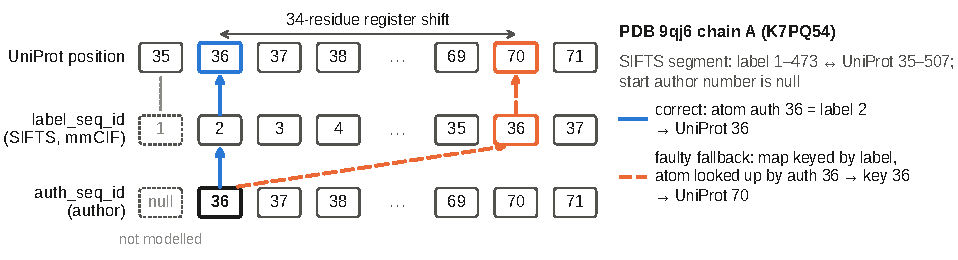
\includegraphics[width=\textwidth]{rev3/f1_mechanism.pdf}
\caption{How the numbering fallback shifted entry 9qj6, chain A. The SIFTS
segment begins at an unobserved residue, so its author number is missing and
the map is built from label numbers. Atoms are then looked up by author
number, which runs 34 ahead, and author residue 36 is paired with UniProt
70 instead of 36.}
\label{fig:mechanism}
\end{figure}

Throughout, the \emph{training-era PDB} means entries released on or before
2018-04-30, and a \emph{segment} is one contiguous stretch of a chain mapped
to UniProt by SIFTS.

\section{Related work}
\label{sec:related}

\paragraph{Leakage in ML for science.} Leakage is a recurring cause of
irreproducible results in machine-learning-based science
\citep{kaufman2012,kapoor2023}, and biology has its own guidance on
validation and splitting \citep{walsh2021dome,whalen2022}. In structural
biology, standard train--test splits were shown to leak through sequence and
structural similarity in protein--ligand affinity prediction
\citep{li2017jcim,volkov2022,li2024lppdbbind,graber2025}, and date-based or
metadata-based splits leave similar overlap in docking
\citep{buttenschoen2024} and protein--protein interaction benchmarks
\citep{bushuiev2024,kovtun2024pinder}. Co-folding methods appear to
memorise ligand poses seen in training \citep{skrinjar2025}.

\paragraph{Exposure in AlphaFold evaluation.} The AlphaFold2 paper evaluated
on PDB chains released after the training cutoff and examined template
similarity \citep{jumper2021}. BETA provides version-specific benchmark sets
with sequence and structure filters \citep{dobson2025beta}. Comparisons of
AlphaFold models with new crystal structures that control for templates
\citep{terwilliger2024}, evidence that AlphaFold reproduces memorised
fold-switched states \citep{chakravarty2024}, and training-set ablations
\citep{ahdritz2024} together indicate that what the model has seen changes
what it predicts.

\paragraph{Conformal prediction for structure.} Split conformal prediction
gives finite-sample marginal coverage under exchangeability
\citep{vovk2005,lei2018,angelopoulos2023}. Residues of the same protein are
not exchangeable with residues of other proteins, and hierarchical data need
their own guarantees \citep{dunn2023,lee2023,barber2023}. CalPro applies
evidential and conformal methods to pLDDT \citep{shihab2026calpro}; we do not
reproduce its results here.

\section{Exposure channels}
\label{sec:channels}

Let $R$ be an experimental reference structure, first released on date $r$,
compared with an AFDB model $M$ of the same UniProt accession. All models in
the preregistered census are AlphaFold2 monomer models (the model files
identify them as ``AlphaFold Monomer v2.0''); a few ATLAS accessions are
served by ColabFold models. We distinguish three ways in which $M$ could
have been informed by $R$ or by structures like it.

\paragraph{Training.} AlphaFold2 was trained on PDB structures released on or
before 2018-04-30 \citep{jumper2021}. If $r$ is on or before that date, $R$
may have been a training example. Training also filtered and sampled chains
by cluster and used self-distillation, so eligibility is an upper bound on
use.

\paragraph{Templates.} At inference time AlphaFold2 searches the PDB for
templates. The human-proteome study reports the PDB and PDB70 snapshots it
used \citep{tunyasuvunakool2021}, and AFDB states that templates were
restricted to structures released before 2021-02-15 \citep{afdbfaq}. AFDB
model files list the PDB entries supplied as templates
(\texttt{\_ma\_template\_ref\_db\_details}), so this channel can be measured
per model. The list records which templates the network was given, not how
much the prediction relied on them.

\paragraph{Homology.} Even when $R$ post-dates both cutoffs, the same protein
or a close homologue may have been in the PDB before the training cutoff.
Release dates do not measure this channel; sequence similarity to the
pre-cutoff PDB does \citep{jumper2021,buttenschoen2024}. Sequence information
also reaches the model through multiple sequence alignments and
self-distillation; we do not measure that.

AFDB entries also carry a \texttt{modelCreatedDate}. AFDB documents it as
the date the entry was created \citep{afdbmetadata}, and in version 6 the
unchanged models received new metadata and the v6 label while their
coordinates were carried over from version 4 \citep{pdbereleasenotes}. It is not a
record of when a prediction ran or what it could see, so we do not use it as
an exposure measure; the census below uses it only to exclude models created
after its start date.

\section{Data and methods}
\label{sec:setup}

\paragraph{ATLAS.} The ATLAS corpus \citep{vandermeersche2024} contains 1{,}938
entry--chain records over 1{,}735 PDB entries and 943 UniProt accessions, of
which 869 have both an AFDB model and a SIFTS mapping
\citep{velankar2013,dana2019}. For each reference we took the initial release
date (the first entry of the mmCIF \texttt{\_pdbx\_audit\_revision\_history}).
One accession has an AFDB record we could not decode, leaving 868 accessions
and 935 accession--entry pairs.

\paragraph{Preregistered census.} Before any label existed, we froze a census
design, its analysis code and its predictions in the project repository and
timestamped them with OpenTimestamps. The design fixes
an AFDB version-6 snapshot at $T_0 =$ 2026-09-11 00:00 UTC and collects, in
weekly batches, X-ray entries at 2.5\,\AA{} resolution or better released
after $T_0$. Models created on or after $T_0$ are excluded. This design does
not add exposure control beyond what any post-2021 release filter gives an
AlphaFold2 model; its value is that every choice in the design was fixed
before any lDDT value was computed. The first four weekly batches (the first
was empty), ending 4 October 2026, produced 488 chain segments from 272
accession--entry pairs and 138 accessions under the original residue mapping
(495 segments and 141 accessions after the correction in
Section~\ref{sec:defect}). We report these four of the 12 planned weekly
batches. The unit of analysis for exposure is
the accession; for labels it is the residue, grouped by chain segment.

\paragraph{Post-2022 census.} An earlier exploratory census of 168 X-ray
entries released after 2022-06-02 used the same pairing code, except that it
discarded pairs whose amino acids differed. We use it to check whether
findings from the preregistered census recur.

\paragraph{Residue pairing and lDDT.} We call the per-residue lDDT values
\emph{labels}. For each reference chain we pair C$\alpha$ atoms with AF
model residues through the PDBe SIFTS UniProt mapping. The corrected
labeller keys the mapping on the label residue number
(\texttt{label\_seq\_id}) and the chain's label identifier
(\texttt{struct\_asym\_id}); maps equal-length segments by offset and
unequal-length segments by global alignment of the entity sequence to the
UniProt sequence; drops any pair whose amino acids differ; and rejects a
segment if more than 10\% of its pairs differ. Chains with fewer than 30
aligned residues are excluded. The label is lDDT-C$\alpha$
\citep{mariani2013}, computed per chain against the AF monomer over aligned
residues, with a 15\,\AA{} neighbour radius and thresholds of 0.5, 1, 2 and
4\,\AA. pLDDT is read from the model's B-factor column and never used to
build labels.

\paragraph{Homology exposure.} For each census accession we queried the RCSB
search service \citep{burley2023} for entries released on or before
2018-04-30 that (i) map to the same UniProt accession, (ii) contain a
polymer at 95\% or higher sequence identity, or (iii) at 30\% or higher
(MMseqs2 \citep{steinegger2017}; e-value $\le 0.1$; query = canonical UniProt
sequence; no query-coverage threshold, so a hit, including a same-accession
hit, may cover only part of the protein). Each accession takes its strongest
class. A failed query leaves an accession unresolved rather than novel; none
failed (Appendix~\ref{app:search}).

\paragraph{Template exposure.} From each AFDB model file the census
downloaded, we read the template PDB IDs, mapped each to UniProt through
SIFTS, and recorded its release date. A model has a same-protein template if
any template maps to its accession.

\paragraph{Registered coverage prediction.} For each of 200 random
protein-level splits (seeds 0--199), 50\% of accessions form a training set
used only to compute the median lDDT $\hat y$, 25\% form the calibration set,
and 25\% the test set. Every residue receives the interval $\hat y \pm q$,
where $q$ is the $\lceil (n_{\mathrm{cal}}+1)(1-\alpha)\rceil$-th smallest
calibration score $|y-\hat y|$ \citep{vovk2005,lei2018}. The interval ignores
pLDDT, so the test concerns the pipeline, not AlphaFold's confidence. We
predicted that mean residue-level test coverage over the 200 splits would be
at least the nominal level minus three Monte Carlo standard errors, at
$1-\alpha = 0.90$ and $0.95$; the MCSE is the standard deviation of coverage
over splits divided by $\sqrt{200}$, so the threshold depends on the data.
Calibration residues are pooled across proteins of very different sizes, and
for such hierarchical data marginal residue-level coverage carries no
finite-sample guarantee \citep{dunn2023,lee2023}.

\section{Most ATLAS references predate the training cutoff}
\label{sec:atlas}

\begin{table}[htbp]
\centering
\caption{Training eligibility of ATLAS references. An accession counts as
training-eligible when every dated reference was released on or before
2018-04-30.}
\label{tab:atlas}
\begin{tabular}{lrrr}
\toprule
Unit & Total & Training-eligible & At least one later reference\\
\midrule
Accessions & 868 & 791 (91.1\%) & 77 \\
Accession--entry pairs & 935 & 851 (91.0\%) & --- \\
\bottomrule
\end{tabular}
\end{table}

Of 868 ATLAS proteins, 791 (91.1\%) are represented only by structures
released on or before AlphaFold2's training cutoff (Table~\ref{tab:atlas}).
The 935 dated references were released between 1988 and 2023, with a median
of 2008.
Agreement between AFDB models and these references cannot by itself be read as
evidence of generalisation; only 77 proteins have any reference released
after the cutoff. Comparing release dates with the AFDB creation date instead
would flag 863 of 868 proteins (99.4\%), a figure that reflects when database
entries were created rather than what the model saw. ATLAS was built to
describe dynamics, not to evaluate AlphaFold; reusing it to study AlphaFold
error needs an explicit exposure control.

\section{A post-cutoff release does not imply an unseen protein}
\label{sec:homology}

\begin{table}[htbp]
\centering
\caption{Exposure of the 138 proteins in the first four batches of the
preregistered census. Homology: strongest relative in the PDB released on or
before 2018-04-30. Templates: what the AFDB model file lists.}
\label{tab:homology}
\begin{tabular}{lrr}
\toprule
Class & Proteins & Share \\
\midrule
\multicolumn{3}{l}{\emph{Homology (training-era PDB)}}\\
Same UniProt accession & 78 & 56.5\% \\
Other entity, $\ge$95\% identity & 9 & 6.5\% \\
Other entity, $\ge$30\% identity & 41 & 29.7\% \\
No relative at $\ge$30\% & 10 & 7.2\% \\
\midrule
\multicolumn{3}{l}{\emph{Templates (AFDB model file)}}\\
Same-protein template & 45 & 32.6\% \\
Other templates only & 88 & 63.8\% \\
Unresolved$^a$ & 5 & 3.6\% \\
\bottomrule
\end{tabular}

\smallskip
\footnotesize $^a$ The SIFTS lookup failed for at least one template, and no
other template maps to the protein.
\end{table}

Every structure in the preregistered census was released after $T_0$, more
than eight years after the training cutoff. Yet 87 of 138 proteins (63.0\%)
had a structure of the same accession or of a 95\%-identical sequence in the
training-era PDB, 128 (92.8\%) had a relative at 30\% identity or more, and
only 10 (7.2\%) had none (Table~\ref{tab:homology},
Figure~\ref{fig:exposure}). Well-studied proteins have many: hen egg-white
lysozyme (P00698) had 730 same-accession entries before the cutoff, human
carbonic anhydrase~2 (P00918) 700, and $\beta_2$-microglobulin (P61769) 693.
These sequence hits show that a related structure existed; they do not say
whether it differs by ligand, mutation, construct or crystal form.

The template records give a more direct measure. All 138 model files list
four PDB templates, released between 1988 and January 2021, none after the
documented 2021-02-15 limit. For 45 proteins (32.6\%) at least one template
is a structure of the same protein; for 88 all templates are other proteins;
for 5 the SIFTS lookup failed for at least one template and no other
template maps to the protein. The two channels overlap but
do not coincide. Of the 78 proteins with a same-accession structure in the
training-era PDB, 43 were given a same-protein template and 35 were not.
Conversely, two proteins with no same-accession structure before the
training cutoff were given one as a template, released in 2019 and 2020;
one of them (Q9F0J8) has no relative at 30\% identity in the training-era
PDB at all.

\begin{figure}[htbp]
\centering
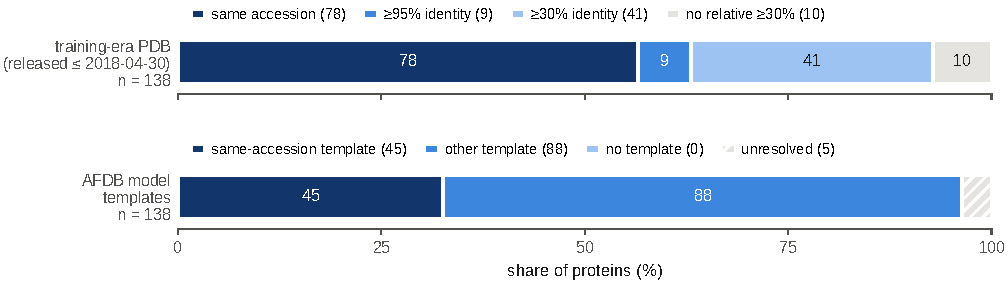
\includegraphics[width=0.85\textwidth]{rev3/f3_exposure.pdf}
\caption{Exposure of the 138 preregistered-census proteins: strongest
relative in the training-era PDB (top) and templates listed in the AFDB model
file (bottom).}
\label{fig:exposure}
\end{figure}

\paragraph{Does exposure change agreement?} Prevalence alone does not show
that exposure matters. As an exploratory check, registered before it was
run, we compared per-protein agreement in the post-2022 census between
proteins with a close training-era relative (same accession or $\ge$95\%
identity) and those without, using each protein's median lDDT and median
pLDDT and averaging over proteins. The 40 proteins with a close relative had
a slightly higher median lDDT than the 45 without (0.975 against 0.959;
difference 0.016, 95\% bootstrap interval 0.003 to 0.032), but also a higher
median pLDDT (96.1 against 92.3; difference 3.8, interval 1.7 to 6.0). The
per-protein share of confident errors (pLDDT $\ge$ 90 and lDDT $<$ 0.60) was
the same in both groups (0.12\% and 0.13\%; difference $-0.01$ percentage points,
interval $-0.18$ to $0.17$). At this sample size, proteins with close
relatives are predicted somewhat better and pLDDT reflects this; we see no
sign that exposure distorts pLDDT calibration, but the comparison could not
detect a small effect. We did not run this
comparison on the preregistered census, where pLDDT-conditional coverage is
the subject of registered predictions that have not yet been evaluated.

\section{A residue-numbering error that manufactured confident errors}
\label{sec:defect}

\subsection{Mechanism}

PDBe's SIFTS mapping gives, for each segment of a chain, its start and end
in \texttt{label\_seq\_id} numbering and, when that residue was observed, in
author (\texttt{auth\_seq\_id}) numbering. Our census code built each
residue map from the author number and fell back to the label number when
the author number was missing, which happens whenever the first residue of a
segment is unobserved. Atoms were then looked up by author number. When the
two schemes differ by an offset, every residue of the segment is paired with
the wrong UniProt position. No per-residue identity check was in place to
catch it.

Figure~\ref{fig:mechanism} shows entry 9qj6, chain~A, of K7PQ54
(dihydrolipoyl dehydrogenase from the lesser grain borer, 507 residues). The
SIFTS segment starts at label residue~1, UniProt~35, which is unobserved.
Author numbering runs 34 ahead of label numbering, so the atom with author
number~36 (label~2, UniProt~36) was assigned UniProt~70. Under this shift
the chain's median lDDT was 0.198 (chain~B: 0.199) at a median pLDDT of
98.4. With the mapping fixed, 472 and 471 residues align with no sequence
mismatch and median lDDT 0.993 and 0.995.


\subsection{Scope}

We replayed the census from its stored, hash-checked source files with the
original and the corrected labeller. With the original labeller the replay
reproduced every stored batch exactly, which confirms that it re-executes
the registered pipeline. Table~\ref{tab:scope} compares the two label sets.

\begin{table}[htbp]
\centering
\caption{The first four batches of the preregistered census, labelled with the
original and the corrected residue mapping.}
\label{tab:scope}
\begin{tabular}{lrr}
\toprule
 & Original & Corrected \\
\midrule
Residue rows & 117{,}905 & 123{,}454 \\
Chain segments & 488 & 495 \\
Accessions & 138 & 141 \\
Residues with lDDT $<$ 0.60 & 31.9\% & 1.1\% \\
High-confidence, low-accuracy chains$^a$ & 116 & 0 \\
K7PQ54 chains with median lDDT $<$ 0.4 & 29 of 38 & 0 of 38 \\
\bottomrule
\end{tabular}

\smallskip
\footnotesize $^a$ At least 30 residues, median pLDDT $\ge$ 90 and median
lDDT $<$ 0.4; the 116 chains span 32 accessions.
\end{table}

Of the 488 original chain segments, 188 changed in median lDDT and 151,
across 40 accessions, changed by more than 0.2
(Figure~\ref{fig:scope}). The share of residues below 0.60 lDDT fell from
31.9\% to 1.1\%. After correction no chain combines high pLDDT with low
lDDT, and none of the 13 entries whose chains had disagreed with each other
by 0.4 or more in median lDDT still does. K7PQ54 alone contributed 14\% of the original rows
and half of the misses at the 0.90 level. The corrected set is not a subset
of the original: it labels 6{,}465 residue positions that the original did not
and drops 916 that it did (a net gain of 5{,}549), and it
adds three accessions and seven segments that the original mapping had
rejected. An independent audit with a
separately written parser and lDDT implementation reproduced the corrected
labels of 36 sampled segments exactly.

\begin{figure}[htbp]
\centering
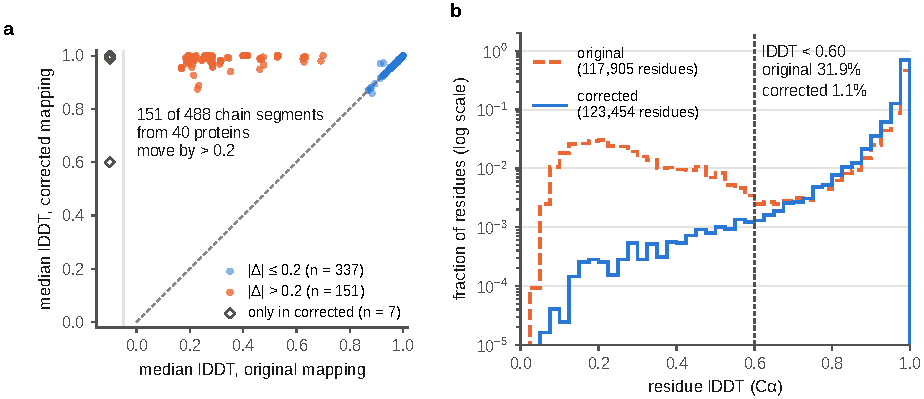
\includegraphics[width=\textwidth]{rev3/f2_scope.pdf}
\caption{Effect of the correction on the first four batches. (a) Median lDDT
per chain segment with the original (x) and corrected (y) mapping; the
dashed line marks no change, and segments that changed by more than 0.2 are
shown in orange. Diamonds at the left are the seven segments that only the
corrected mapping labels. (b) Distribution of residue-level lDDT with each
mapping (logarithmic scale).}
\label{fig:scope}
\end{figure}

\subsection{Why it was dangerous, and how it could have been caught}

The error did not add noise. It created residues that AlphaFold was
confident about and that appeared to be badly wrong, which is the signature
of overconfidence. A calibration study run on these labels could have
reported that AlphaFold is overconfident on new structures, and our
registered coverage test did fail on these labels. The registration and the
stored source files are what let us trace the failure to the labels rather
than to the model.

The precondition is common: 304 of the 492 SIFTS segments mapped to these
proteins (62\%) begin on an unobserved residue. It becomes an error only when
author and label numbering are offset, which was the case for 147 segments
(30\%) from 39 proteins, with offsets from $-31$ to $+201$. In a comparison
we added after the fact, all 147 were among the 151 segments whose median
lDDT changed by more than 0.2; in the other four the offset changes within
the segment.

The direct test is an amino-acid identity check on every pair: under a
register shift almost no paired residues match, which is why the post-2022
census, which discarded mismatched pairs, lost data instead of corrupting it
(Section~\ref{sec:post2022}). Coarser checks catch some cases. A third of
residues below 0.60 lDDT is far from the 2.6\% seen in the corrected
post-2022 census,
and 13 entries had chains of the same protein that disagreed by 0.4 or more
in median lDDT. A chain-agreement check would still miss entries such as
9qj6, where both chains were shifted alike.

\subsection{The same error in the post-2022 census}
\label{sec:post2022}

Because the post-2022 census discarded pairs whose amino acids differed, the
error there mostly removed data rather than corrupting it: of 168 entries, 69
were rejected for having too few aligned residues and 3 because the model
could not be downloaded. With the corrected mapping, 45 of those 69 produce
labels, and 139 entries in all instead of 96 (37{,}531 residue rows instead of 24{,}457). The rank correlation between
pLDDT and lDDT rose from 0.617 to 0.643. Among residues with pLDDT $\ge$ 90,
the share below 0.60 lDDT halved, from 0.58\% ($n = 20{,}777$) to 0.29\%
($n = 31{,}032$), while in the lowest-confidence bin (pLDDT $<$ 50) it rose
from 58\% ($n = 177$) to 75\% ($n = 314$). Most of these changes come from
the 45 newly labelled entries; residues that matched by chance under a shift,
and so passed the identity filter, account for a smaller part (for example
in entry 10ke). This relabel is exploratory. It used source files fetched
again in October 2026, because the September files had not been kept, whereas
the preregistered census was replayed from its original stored files.

\subsection{The registered coverage prediction, before and after}

\begin{table}[htbp]
\centering
\caption{Registered coverage prediction on the original and corrected
labels: mean residue-level test coverage over 200 protein-level splits and the
threshold, nominal minus three Monte Carlo standard errors. The prediction
fails on the original labels and holds on the corrected labels.}
\label{tab:p5}
\begin{tabular}{lcccc}
\toprule
 & \multicolumn{2}{c}{Original labels} & \multicolumn{2}{c}{Corrected labels}\\
\cmidrule(lr){2-3}\cmidrule(lr){4-5}
Nominal & Mean coverage & Threshold & Mean coverage & Threshold \\
\midrule
0.90 & 0.8580 & 0.8760 & 0.8945 & 0.8914 \\
0.95 & 0.9152 & 0.9328 & 0.9456 & 0.9449 \\
\bottomrule
\end{tabular}
\end{table}

On the original labels the prediction failed at both levels
(Table~\ref{tab:p5}). Those labels were corrupted, and we retract the result;
the original outputs remain archived unchanged. On the corrected labels
(123{,}454 residues from 141 accessions, against 117{,}905 from 138 before)
the prediction holds at both levels. At 0.90 the mean exceeds the threshold by
0.0031, about one Monte Carlo standard error; at 0.95 it does so by 0.0007,
less than half of one (MCSE 0.0017), so this level passes only narrowly. A
margin this small could reverse under a different but equally defensible
repair. It does not reverse when residues on the interval boundary are counted
as uncovered (0.9453 against 0.9449).

The rerun is not blind. Before registering it we computed the same statistic
outside the registered pipeline on a preliminary version of the repair
(122{,}024 residues rather than 123{,}454) and obtained 0.898 and 0.947. The seeds
and decision rule were fixed by the original registration (the thresholds
depend on the data only through the MCSE), and the repair rule was registered before the
rerun. The rerun used the registered evaluator, called directly because
data collection was paused while the error was fixed. An
independent reimplementation that shares no code with the evaluator
reproduced both means exactly and, on the original labels, the original
failure. The original failure is therefore consistent with a labelling
artefact. Because the interval ignores pLDDT, the result is consistent with
sound labels and a sound pipeline; it says nothing about how well pLDDT tracks error.

\section{Recommendations}
\label{sec:recommendations}

\begin{enumerate}
\item Report training eligibility, template exposure and homology exposure
      separately, and state which ones the question requires to be
      controlled. Release dates and database creation dates are not exposure
      measures.
\item For AFDB models, read the template list from the model file; it is
      available and cheap to extract.
\item Stratify results by sequence similarity to the training-era PDB, as
      leakage-aware benchmarks already do.
\item Key residue correspondences on a single numbering scheme, bind them to
      the chain identifier, and assert amino-acid identity for every pair.
\item Sanity-check label distributions against pLDDT and between chains of
      the same entry before running any downstream analysis.
\item Register analyses before labels exist and keep the raw inputs, so
      that an error found later can be replayed and corrected rather than
      argued about.
\end{enumerate}

\section{Limitations}
\label{sec:limitations}

First, the census models are AlphaFold2 monomer models; other versions and
AlphaFold3 \citep{abramson2024} have their own cutoffs. Second, template
lists record what the network was given, not what it used, and we did not
measure sequence-level exposure through alignments or self-distillation.
Third, homology was measured with fixed identity thresholds, a single
canonical sequence and no coverage threshold, so a 30\% hit can be a short
domain match. Fourth, labels compare single chains with monomer models, so
interfaces and ligands in the crystal are ignored. Fifth, the preregistered
census is reported after four of its 12 weekly batches (138 proteins, 10
without a relative), and the full cohort may differ. The corrected label set
also differs from the original (6{,}465 residue positions
gained, 916 lost). Finally, the
post-2022 relabel was run on re-fetched source files, which may differ from
those used originally.

\section{Conclusion}

In both corpora we examined, most proteins were exposed in at least one
channel. Exposure has to be measured channel by channel; the template lists in
AFDB model files make one of those channels directly observable. Residue
correspondence deserves the same care. In our case a single numbering fallback
was enough to make accurate predictions look like confident errors and to
make a registered coverage prediction fail; on corrected labels the same
prediction holds, narrowly at the 0.95 level. The registration and the stored inputs let us find the
cause and undo it.

\appendix

\section{Provenance}
\label{app:provenance}

\begin{table}[h]
\centering
\caption{Timeline of the preregistered census and its correction.}
\label{tab:timeline}
\begin{tabular}{ll}
\toprule
Date (2026) & Event \\
\midrule
9 Sep & Design, analysis code and predictions frozen (Bitcoin timestamp confirmed 10 Sep) \\
11 Sep & Snapshot instant $T_0$ \\
4--5 Oct & Batch-4 evaluation records the coverage failure \\
7 Oct & Independent audit traces 9qj6 to the numbering fallback; collection paused \\
7 Oct & Repair, replay protocol and correction registered before rerunning \\
7 Oct & Replay of batches 1--4 with both labellers; post-2022 census relabelled \\
7 Oct & Independent audit of repair, replay and relabel \\
9 Oct & Registered rerun on corrected labels completes; independent recomputation \\
\bottomrule
\end{tabular}
\end{table}

Internally the analyses are numbered e420 (ATLAS), e421 (post-2022 census),
e422 (preregistered census) and e427 (repair and replay). Registrations and
checkpoints carry SHA-256 digests timestamped with OpenTimestamps.

\section{Homology search details}
\label{app:search}

Queries used the RCSB Search API \citep{rcsbsearchapi}. Every request and
response was cached with its SHA-256 digest. The API returns HTTP 204 for a
query that ran and found nothing; across the 224 accessions queried for both
censuses, 594 queries returned 200, 408 returned 204, and none failed.

\section*{Data and code availability}

The registrations with their timestamp proofs, the analysis code, the derived
residue-level tables and the request digests are available at
\url{https://github.com/MachineLearning-Nerd/afdb-exposure-audit}, together
with a script that recomputes every number in this paper from them. The full
evaluation records of the preregistered census, which contain predictions
that are still blind, will be added when the census closes. Raw files from the PDB, AFDB,
PDBe/SIFTS, UniProt and ATLAS are not redistributed; each can be re-fetched
from its public source, and the SHA-256 digests recorded with every request
identify the exact bytes used. The preregistered census was replayed from its
original stored files; the post-2022 relabel used files fetched again in
October 2026 (Section~\ref{sec:post2022}).

\bibliographystyle{plainnat}
{\raggedright
\bibliography{references}
}

\end{document}
